\section{Preliminary Work}

\subsection{Token Analysis}
Prior research in computer networking hints that we should expect network configurations to share a common set of tokens. In~\cite{complexity} researchers identified a few key design decisions commonly made by network operators. Network configurations are designed to be homogeneous as a means of easy maintenance, where some operators start off with common configuration templates with varying parameters. They may then tweak these templates to achieve specialized routing roles if needed. Thus one can posit that configurations across devices in a given network may share a lot of the same tokens, subnets and sometimes even complete stanzas (such as Access Control Lists).\\ 

To confirm our hypothesis, we took configurations from a few sample networks and split up each configuration file into a list of tokens. Tokens included all keywords and subnets with punctuation and newline characters stripped off. For every file we then plotted the percentage of tokens that exist in other router configuration files.

\begin{figure}[H]
	\centering
	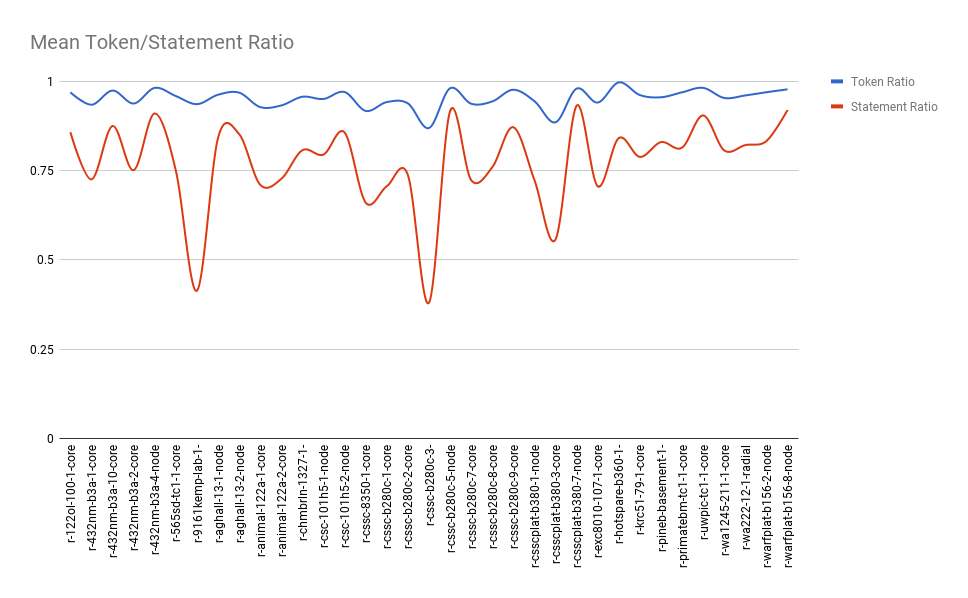
\includegraphics[width=\textwidth]{chart.png}
	\caption{The plot shows how many tokens and statements a router configuration holds in common with the rest of the network. The data was taken from a large research university.}
\end{figure}

Our results show that most files could be rebuilt from existing statements in routing configurations due to the amount of tokens they share. Given our results, and the observations made by~\cite{complexity} about how networks are configured, we can confidently hypothesize that most token suggestions can be generated from analyzing other existing configurations. This effectively makes all router configuration histories a part of the search space for our NLP model. 

\subsection{Model Construction}
During the semester, we developed a program in Python which builds a bigram model out of input files. We use the NLTK package [cite] to build the model. The package also allows us to easily incorporate likelihood ratios as a means of scoring the bigrams. Our script was run on sample configurations from the ARC package. These configurations are simple in nature but mimic what deployed network configurations would look like. Each set of configurations emulates a small network employing a different routing policy or design. This allows for a wide breadth of network configuration types to be considered for our model. We incorporated some preprocessing steps to clean up the data. Since IP addresses and subnets tend to vary a lot and add noise to the data, we replaced them with placeholders. In the future work section, we consider other approaches to help suggest IP addresses.\\

To test the accuracy of our model, we perform Leave One Out (LOO) Cross Validation. This form of cross validation involves using one observation as the validation set and the remaining observations as the training set. This is repeated for all combinations of training sets, allowing every observation to act as a validation set. For our analysis an observation is one set of configurations. For example, consider five set of configurations: A through E. We pick A as the validation set and train the model on all other configurations. Our program will now “walk through” rebuilding configuration A, starting from the first keyword. At every step, we invoke our model and compare our predictions against the actual tokens in A. If the model generates the correct prediction within the top three results, we mark a token completion to be successful.\\
 

\begin{figure}[H]
	\centering
	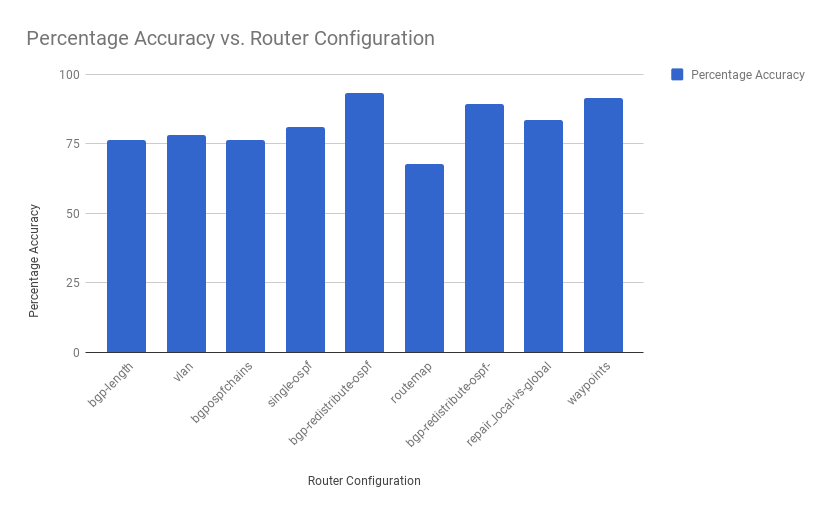
\includegraphics[width=\textwidth]{model_analysis.png}
	\caption{The bar charts show the accuracy of the model for each set or router configurations used as the validation set.}
\end{figure}
Since we had 10 sets of configurations at our disposable, we performed 10 LOOs and took the average of the accuracies for a final accuracy measure. Our results are promising and we see accuracies of up to 93\%, and an average of 81\%.